%************************************************
%\chapter{Outlook: Observation of a time crystal in the Rydberg Experiment?}
%Novel stabilization mechanisms due to disorder?
%
%Preliminary results show a time crystalline signature in the Rydberg experiment but pure pair model does not find this. However there also random on-site potentials due to van-der Waals interactions, these 
%
%\texttt{rydberg-pair-timecrystal.jl}
%Replace interacting Hamiltonian with Pair model. Then dynamics are effectively average over pair  distribution. Each pair is not stable but has some lifetime depending on its interaction strength. Since distribution is very broad there is some phase-wrapping going on which leads to a slow decay. So pair model predicts not a stable time crystal but an anomalously slow decay (stretched exponential again?).

\chapter{Conclusion}\label{ch:floquet-discussion}

In Part 2 of this thesis, we have demonstrated time-crystalline behavior shares a close relationship not only to disordered interactions but also to disorder in the driving part.  This insight could be useful in understanding whether the experimental system of Part 1 could potentially show stable time-crystalline signatures. Preliminary experimental results indicate that interactions indeed appear to stabilize the magnetization dynamics of a spatially disordered XX model under repeated imperfect flips about its $x$-axis (cf. Fig.~\ref{fig:rydberg-timecrystal-experiment}). However, a naive calculation in the pair model does not find any true stabilization and instead predicts a decay of the magnetization's envelope on a timescale $\propto\epsilon^2$~\footnote{Note that the graphic uses a different definition for the rotation angle. It uses $\phi=\epsilon \pi$ and thus $\epsilon = 1$ is the soluble point. In contrast this thesis uses $\phi=(1-\epsilon)\pi$ with $\epsilon=0$ being soluble.}. The reason the continuous slow decay are in the end the pairs themselves: Since the system essentially decomposes into non-interacting two-spin subsystems each decaying on a timescale $\propto \epsilon^2/J$, taking the thermodynamic limit cannot cause stabilization. In part this is also due to phase-wrapping effects, which limits a pair's interaction strength $J$ effective to the interval $[0,\pi]$. Since it is so far unclear whether this system is truly a time-crystal or not, we can explore other mechanism in search for potential stabilization. 

\begin{figure}[htb]
	% TODO
	\centering
	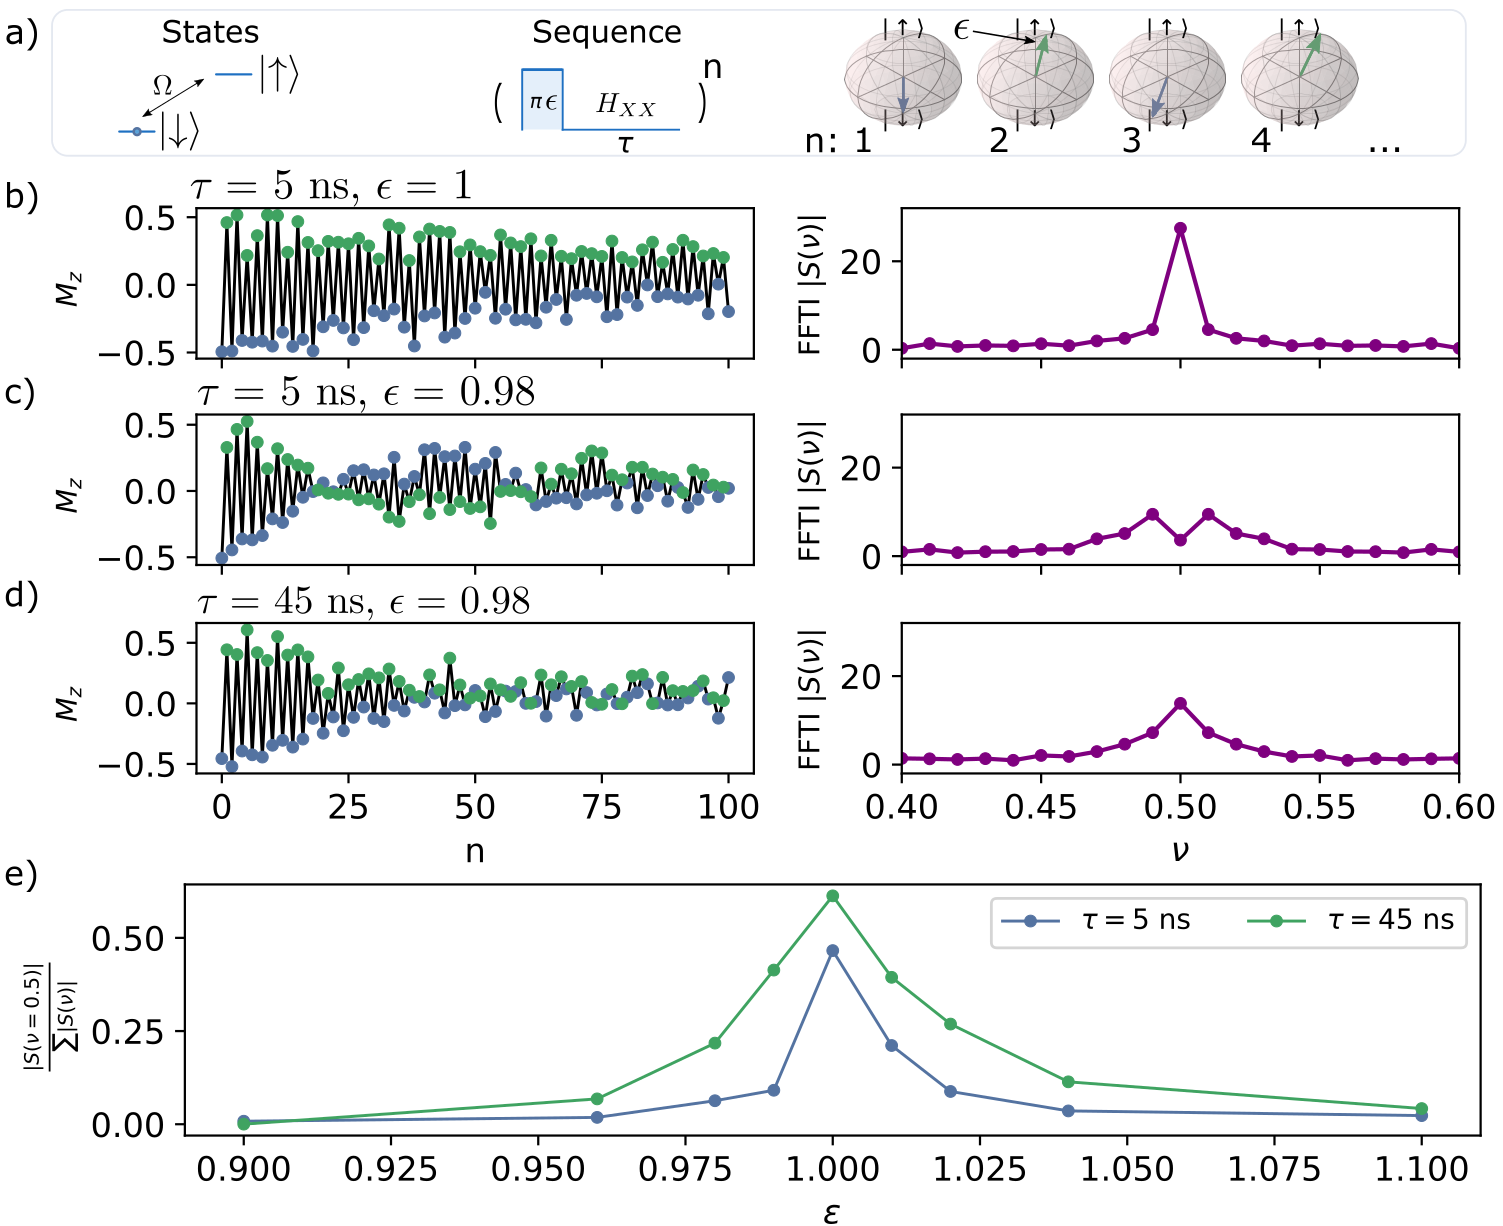
\includegraphics[width=\textwidth]{gfx/preliminary-timecrystal.png}
	\caption{Preliminary experimental results on time-crystalline signatures in a spatially disordered XX model. a) sketches the experimental sequence. Then experimental results for perfect rotation (b), short interaction times and imperfect rotation (c) and longer interaction times with imperfect rotation (d) follow. Left column depict the magnetization's time trace, while right column shows the Fourier transform of the signal. e) Then plots the normalized Fourier weight at $\nu=0.5$ versus rotational deviation $\epsilon$. Taken with permission from Ref.~\cite{geierShapingHamiltonianManybody}}
	\label{fig:rydberg-timecrystal-experiment}
\end{figure}

One unexplored route is the influence of van der Waals interactions which effectively cause locally varying $z$-fields. One way to interpret these is that they change the alignment of the driving field spatially. As we have seen in this part of the thesis, such a spatially varying driving field can help stabilizing time crystalline dynamics.

Another exciting avenue to follow is to consider the interactions among pairs. As we derived in Chapter~\ref{sec:universal-dynamics}, for an XXZ model, these pair-pair interactions take the form of an effective Ising model. Since Ising models as the prototypical example for time crystals, we deem this a very promising approach in the case of XXZ models. However, in XX models this effective Ising term does not exists to first order. So in order to access stabilization effects due to pair-pair interactions a better understanding of the higher orders of the perturbation theory is required.



